\documentclass[12pt]{article}
\usepackage{indentfirst}
\usepackage{fullpage}
\usepackage{multicol,multirow}
\usepackage{tabularx}
\usepackage{ulem}
\usepackage[utf8]{inputenc}
\usepackage[russian]{babel}
\usepackage{listings}
\usepackage{color}
\usepackage{graphicx}
\DeclareGraphicsExtensions{.png}

\begin{document}
\begin{titlepage}
	\begin{center}
		\bfseries
		
		{\Large Московский авиационный институт\\ (национальный исследовательский университет)
			
		}
		
		\vspace{48pt}
		
		{\large Факультет информационных технологий и прикладной математики
		}
		
		\vspace{36pt}
		
		
		{\large Кафедра вычислительной математики и~программирования
			
		}
		
		
		\vspace{48pt}
		
		Курсовая работа по курсу <<Дискрeтный анализ>>: Методы сжатия данных
	\end{center}
	
	\vspace{72pt}
	
	\begin{flushright}
		\begin{tabular}{rl}
			Студент: & В.\,В. Гринин  \\
			Преподаватель: & Н.\,А. Зацепин \\
			Группа: & М8О-408Б \\
			Дата: & \\
			Оценка: & \\
			Подпись: & \\
		\end{tabular}
	\end{flushright}
	
	\vfill
	
	\begin{center}
		\bfseries
		Москва, \the\year
	\end{center}
\end{titlepage}

\pagebreak

\subsection*{Условие}

Необходимо реализовать два известных метода сжатия данных для сжатия одного файла. 

Формат запуска должен быть аналогичен формату запуска программы gzip, должны быть поддержаны следующие ключи: -c, -d, -k, -l, -r, -t, -1, -9. Должно поддерживаться указание символа дефиса в качестве стандартного ввода.

\subsection*{Метод решения}

Метод запуска аналогичен запуску утилиты gzip с небольшой поправкой на то, что программа требует предварительно ввести <<./>>.

\subsubsection*{Обработка входных данных}

Первоначально программа обрабатывает то, что получает на входе, отделяя имена файлов и директорий от введённых ключей. Ключи от файлов программа отделяет по первому символу слова: если этот символ является <<->>, то полученное слово является набором ключей. В процессе изучения поведения утилиты gzip я вывел следующее дерево приоритетов ключей:

\begin{figure}[h!]
	\centering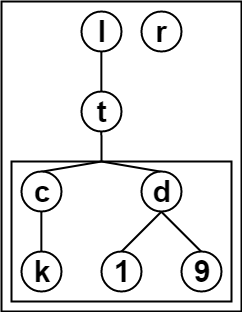
\includegraphics[scale=0.5]{KeyTree}
\end{figure}

Т. е. если уже был введён ключ -t, то далее ключи -c, -k, -d, -1, -9 программа учитывать не будет, но если вы ввели ключ -l, то он делает ключи -c, -k, -d, -t, -1, -9 недействительными как сейчас, так и при их будущих вводах. В то же время сочетания -cd, -c1, -c9, -kd, -k1, -k9, а так же сочетания ключа -r со всеми остальными ключами не являются взаимоисключающими. Если же во время обработки ключей встречается неизвестный ключ, то программа прекращает свою работу с соответствующей ошибкой, как и утилита gzip.

В случае если начальным символом не является <<->>, то оно заносится в красное дерево имён файлов/директорий. В случае если поступивший файл начинается с символа <<->>, файл необходимо ввести через <<./>>.

\subsubsection*{Работа с файлами}

Изначально проверяется пустота дерева имён файлов/папок. Изначально элемент проверяется как директория, и если он ей является, то проверяется активность ключа -r: ключ активирован -- идёт работа с директорией, нет -- пропуск файла; если, поступивший объект не директория, то он автоматически расценивается как файл, и идёт работа с файлом.

Если же дерево пустое то программа завершается.

\subsubsection*{Препроцессинг компрессии}

Если введённые ключи говорят о необходимости компрессии, то при отсутствии ключа -c производится проверка на наличие у файла суффикса <<.gz>>. Если он присутствует, то файл не обрабатывается, и выводится соответствующее сообщение. Если же у этого файла нет расширения <<.gz>>, то при отсутствии ключа -c проверяется наличие файла, имя которого отличается от полученного только стоящим в конце суффиксом. Если такой файл не найден, то работа продолжается. Если же он найден, то пользователю предлагается сделать выбор - перезаписывать данный файл или нет. В случае отрицательного ответа работа с данным файлом прекращается. Далее, при отсутствии ключей -1 и -9 поочерёдно происходит компрессия файла с помощью обоих алгоритмов компрессии (они будут описаны ниже вместе с алгоритмами декомпрессии). В случае провала любого алгоритма компрессии работа с файлом прекращается, и выводится соответствующая ошибка. Если же оба алгоритма сработали нормально, то при отсутствии ключа -c выбирается временный файл, созданный алгоритмами, с меньшим размером, и именно он получает расширение <<.gz>>, а файл с большим размером удаляется. Так же проверяется наличие ключа -k. При его отсутствии изначальный файл удаляется. При наличии ключей -1 или -9 отличия заключаются в том, что применяется только один из алгоритмов: -1 -- LZW, -9 -- арифметическое кодирование.

\subsubsection*{Препроцессинг декомпрессии}

Если же ключи указывают на необходимость декомпрессии, то в случае отсутствия ключа -c и наличии ключа -d проверяется наличие у файла суффикса <<.gz>>. При выполнении всех этих условий работа с файлом прекращается, и выводится соответствующее сообщение. Далее при отсутствии ключей -t и -c проверяется наличие файла с таким же именем, но без расширения <<.gz>>. Если такой файл есть, то пользователю предлагается сделать выбор о его перезаписи. В случае отказа, работа с данным файлом прекращается, и выводится соответствующее сообщение. Если ответ положительный или такого файла нет, то работа продолжается. Из поступившего архива считывается первый байт, который содержит указание на метод архивации. Если этот байт интерпретируется как символ <<L>> или <<A>>,то декомпрессия производится по алгоритму LZW или Арифметика соответственно. Если первый байт интерпретируется иначе, то работа с файлом прекращается, и выводится соответствующее сообщение. В случае неудачного завершения алгоритма, выводится соответствующее сообщение и при отсутствии ключей -t и -c удаляется файл, в который записывались данные после декомпрессии, и работа с файлом прекращается. Далее при отсутствии ключей -t, -c и -k, удаляется изначальный архив, а при отсутствии ключей -t и -c временный файл для декомпрессии переименовывается и получает имя изначального архива без расширения <<.gz>>.

\subsubsection*{Получение информации об архиве}

В случае указания ключа -l производятся следующие действия. Читается первый байт, и в случае, если он не совпадает с буквами, указывающими на метод архивации, то работа прекращается, и выводится соответствующее сообщение. Далее читается 8 байт, в которые помещается размер файла до компрессии. После программа считывает размер архива, и вычисляется процент сжатия. Далее выводятся размер сжатого файла, размер до компрессии, процент сжатия в полуинтервале $[-100\%; 100\%)$ и имя файла до архивации (если файл имеет расширение <<.gz>>, то имя выводится без этого расширения, в противном случае выводится имя архива).

Далее незакодированный файл будет упоминаться как файл, а закодированный файл как архив.%TODO возьмите на вооружение

\subsubsection*{LZW компрессия}

Компрессия методом LZW происходит по следующему принципу: из размера файла определяется верхняя граница буфера, в котором будут храниться слова, и каким количеством байт будут кодироваться слова, после чего строится префиксное дерево из всех односимвольных слов--символов ASCII. Дальнейший процесс компрессии будет описан для случая записи в архив, но процесс вывода результатов в стандартный вывод аналогичен (как и в случае декомпрессии). В архив записывается 9 байт информации, первый из которых - это указание метода архивации, а остальные 8 - размер изначального файла. Если поступивший файл имеет размер $0$, то компрессия прекращается. Далее читается первый символ файла, и в архив записывается код соответствующего слова. Полученный символ указывает на узел, в который будет добавлен следующий символ. Затем символы считываются до создания новой вершины в префиксном дереве, а в архив записывается код вершины, предшествующей новой. Последняя буква, полученная до добавления вершины заносится в буфер. После чего из корня ищется вершина, к которой ведёт эта буква, и процесс повторяется вплоть до окончания символов в файле или создания максимального количества вершин, которое сможет прочитать декомпрессор. Если произошло второе, то в архив записывается $0$, (никак иначе на этом этапе он быть записан не может), ранее установленным количеством байт, из префиксного дерева удаляются все вершины кроме корневой и потомков первого рода, после чего процесс компрессии начинается заново, но позиции в исходном файле и архиве не получают откат. Если на каком либо этапе компрессии возникает ошибка, его работа прекращается, и выводится соответствующая ошибка.

\subsubsection*{LZW декомпрессия}

Декомпрессия начинается с прочтения размера изначального файла из архива, который необходим для определения нужно количества байт для прочтения слова и проверки на безошибочность декомпрессии. Далее, из архива считываются только коды слов определённого ранее размера. После считывания первого слова создаётся красно-чёрное дерево, и в него записываются все односимвольные слова из ASCII символов. Далее, по полученному коду в дереве находится необходимая строка, и она записывается в файл. После чего этот символ записывается во временное слово. Далее алгоритм считывает коды из архива. При обработке кодов возможны 4 ситуации:

\begin{enumerate}
	\item Код входит в список полученных слов. В этом случае в красно-чёрном дереве ищется слово с необходимым кодом, и это слово записывается в файл, после чего в красно-чёрное дерево записывается новое слово, которое является предыдущим словом, к которому добавили первую букву только что полученного. Декомпрессия продолжается.
	\item Код не входит в красно-чёрное дерево, но он является следующим по счёту, следовательно это слово можно интерпретировать как предыдущее, к которому дописали в конце букву, с которой оно начинается. Полученное слово записывается в файл и в красно-чёрное дерево, после чего декомпрессия продолжается.
	\item Код не входит в красно-чёрное дерево и не является следующим на подходе, следовательно архив повреждён. Декомпрессия прекращается, и выводится соответствующее сообщение.
	\item Код равен $0$. Красно-чёрное дерево очищается, и процесс декомпрессии начинается сначала, но позиции в файле и архиве не получают откат.
\end{enumerate}

По окончании чтения архива, количество байт, которое было в изначальном файле, сверяется с тем, сколько было записано в его новую версию. При несовпадении выводится соответствующее сообщение, и декомпрессия завершается неудачно.

%TODO куда записать принцип рабты с файлами? и напишите ниже про свои алгоритмы

\subsubsection*{Арифметическая компрессия}

\subsubsection*{Арифметическая декомпрессия}

\subsection*{Описание файлов программы}

Код программы разбит на 13 файлов:

\begin{enumerate}
	\item Arithmetic.h - Содержит перечисление методов и описание класса TArithmetic, необходимого для работы арифметической компрессии и декомпрессии. 
	\item Arithmetic.cpp - Содержит реализацию всех методов класса TArithmetic.
	\item BFile.h - Содержит перечисление методов и описание класса TOutBinary и класса TInBinary, необходимых для записи в файл и чтения из файла соответственно.
	\item BFile.cpp - Содержит реализацию всех методов классов TOutBinary и TInBinary.
	\item Globals.h - Содержит в себе все необходимые глобальные переменные и библиотеки используемые несколькими файлами.
	\item LZW.h - Содержит перечисление методов и описание класса TLZW, необходимого для работы алгоритма LZW.
	\item LZW.cpp - Содержит реализацию всех методов класса TLZW.
	\item main\_help.h - Содержит в себе перечисление и описание всех функций необходимых для препроцессинга перед началом работы алгоритмов компрессии и декомпрессии.
	\item main\_help.cpp - Содержит реализацию всех функций, необходимых для препроцессинга, описанных в файле main\_help.h.
	\item TPrefix.h - Содержит перечисление методов и описание класса TPrefix, необходимого для работы LZW компрессии.
	\item TPrefix.cpp - Содержит реализацию всех методов класса TPrefix.
	\item main.cpp - Содержит в себе алгоритм чтения файлов и ключей.
	\item Makefile - Файл для сборки программы.
\end{enumerate}

\subsection*{Основные типы данных}

\begin{enumerate}
	\item TArithmetic - класс, описывающий работу арифметического алгоритма компрессии и декомпрессии.
	\item TOutBinary - класс обеспечивающий запись необходимого количества байт в файл.
	\item TInBinary - класс обеспечивающий считывание необходимого количества байт из файла.
	\item TLZW - класс, описывающий работу алгоритма LZW.
	\item TPrefix - класс, обеспечивающий построение префиксного дерева для LZW сжатия.
\end{enumerate}

\subsection*{Описание методов и функций программы}
 
\subsubsection*{Основные свойства и методы класса TArithmetic}%TODO Слава внимательно посмотрите как я это оформил в своих subsubsection
\noindent
public:

\begin{enumerate}
	\item 
	\item 
	\item 
	\item 
	\item 
	\item 
	\item 
	\item 
\end{enumerate}
\noindent
private:

\begin{enumerate}
	\item 
	\item 
	\item 
	\item 
	\item 
	\item 
	\item 
	\item 
\end{enumerate}

\subsubsection*{Основные свойства и методы класса TOutBinary}%TODO Слава
\noindent
public:

\begin{enumerate}
	\item 
	\item 
	\item 
	\item 
	\item 
	\item 
	\item 
	\item 
\end{enumerate}
\noindent
private:

\begin{enumerate}
	\item 
	\item 
	\item 
	\item 
	\item 
	\item 
	\item 
	\item 
\end{enumerate}

\subsubsection*{Основные свойства и методы класса TInBinary}%TODO Слава
\noindent
public:

\begin{enumerate}
	\item 
	\item 
	\item 
	\item 
	\item 
	\item 
	\item 
	\item 
\end{enumerate}
\noindent
private:

\begin{enumerate}
	\item 
	\item 
	\item 
	\item 
	\item 
	\item 
	\item 
	\item 
\end{enumerate}

\subsubsection*{Основные свойства и методы класса TLZW}
\noindent
public:

\begin{enumerate}
	\item TLZW(TInBinary*, TOutBinary*) - Конструктор класса. Передаются файл для чтения и файл для записи.
	\item bool Compress(std::string) - Производит компрессию данных. На вход получает имя файла для компрессии. В случае успешного выполнения возвращает true, иначе false.
	\item bool Decompress(std::string) - Производит декомпрессию данных. На вход получает имя файла для декомпрессии. В случае успешного выполнения возвращает true, иначе false.
	\item $\sim$TLZW() - Стандартный деконструктор.
\end{enumerate}
\noindent
private:

\begin{enumerate}
	\item TInBinary* ForRead - Файл для чтения.
	\item TOutBinary* ForWrite - Файл для записи.
	\item TPrefix* CompressionTree - Префиксное дерево для хранения слов при компрессии.
	\item std::map<unsigned long long int, std::string> DecompressionTree - Красно-чёрное дерево для хранения слов при декомпрессии.
\end{enumerate}

\subsubsection*{Основные свойства и методы класса TPrefix}

\noindent
public:

\begin{enumerate}
	\item TPrefix(TInBinary*, TOutBinary*) - Конструктор для корневой вершины. Передаются файл для чтения и файл для записи.
	\item TPrefix() - Конструктор для всех прочих вершин.
	\item int Update(char) - Добавление вершины из других вершин. Возвращает коды ошибок или успехов.
	\item int UpdateForRoot() - Добавление вершины из корня. Возвращает коды ошибок или успехов.
	\item void Clear(bool) - Очистка дерева после переполнения.
	\item $\sim$TPrefix() - Стандартный деконструктор.
\end{enumerate}
\noindent
private:

\begin{enumerate}
	\item std::vector<std::pair<char, TPrefix*>\hspace{0pt}> Next - Вектор потомков вершины и путей в них.
	\item unsigned long long int NumberOfWord - Номер слова в данном узле.
	\item static char LastLetter - Последняя прочитанная буква. Необходима для построения нового слова.
	\item static unsigned long long int NeedToRead - Вспомогательная переменная для чтения нужного кол-ва символов.
	\item static unsigned long long int LastNumber - Номер следующего добавленного слова.
	\item static unsigned long long int Border - Максимальная граница количества слов перед очисткой дерева.
	\item static TInBinary* ForRead - Файл для чтения.
	\item static TOutBinary* ForWrite - Файл для записи
	\item static unsigned short int Bites - Количество байт, необходимое для кодирования слова.
\end{enumerate}

\subsubsection*{Прочие функции}
\noindent
\begin{enumerate}
	\item bool KeyManager(std::string) - Обрабатывает полученные ключи. В случае получения неизвестного ключа возвращает false, иначе true.
	\item bool DifferensOfSizes(TInBinary*, std::string) - вывод для каждого файла размера сжатого, оригинального, коэффициента сжатия(\%) и имя оригинального файла(ключ l). В случае повреждения. архива возвращает false, иначе true.
	\item void WorkWithDirectory(std::string) - работает с директорией (ключ r).
	\item void WorkWithFile(std::string) - работает с файлом (определяет наличие файла, принимает решение о компрессии или декомпрессии, выполняет прочие ключи).
	\item bool IsDirectory(std::string, bool) - Проверяет, является ли файл директорией. Если файл является директорией, возвращает true, иначе false.
	\item void PrintDirectoryErrors(std::string) - Уведомляет об ошибках.
	\item bool IsArchive(std::string) - Проверяет, является ли файл архивом. Если файл является архивом, возвращает true, иначе false.
	\item void Rename(std::string, std::string) - Изменяет название файла после успешной компрессии или декомпрессии.
	\item void Delete(std::string) - Удаляет временный файл.
	\item void MainDecompress(TInBinary*, std::string) - Отвечает за подготовку декомпрессинга.
	\item void MainCompress(TInBinary*, std::string) - Отвечает за подготовку компрессинга.
	\item unsigned long long int LZWCompress(TInBinary*, std::string, TOutBinary*) - Подготавливает LZW компрессию. Возвращает размер нового файла.
	\item unsigned long long int ArithmeticCompress(TInBinary*, std::string) - Подготавливает арифметический компрессию. Возвращает размер нового файла.
	\item void KeepSmall(unsigned long long int, unsigned long long int,%TODO доковырять её
	unsigned long long int, std::string) - Сохраняет архив самого малого размера.
	\item int main(int, char*) - Осуществляет чтение входных данных.
\end{enumerate}

\subsection*{Исходный код}%TODOпоходу его будем вставлять как всё закончим

\subsection*{Тест производительности}%TODO

В качестве теста производительности использовался файл размером%TODO
, наполненный случайными символами английского алфавита.

\noindent
\begin{tabular}{| l | l | l | l | l | l |}
	\hline
             & Размер     & Эффективность & Максимальное & Время      & Время  \\
             & сжатого    & сжатия        & потребление  & компрессии & декомпрессии  \\
             & файла (б) &               & памяти (Мб)  & (с)        & (с) \\
 \hline
 gzip        & & & & & \\
 \hline
 Оба         & & & & & \\
 алгоритма   & & & & & \\
 \hline
 LZW         & & & & & \\
 \hline
 Арифм.      & & & & & \\
 кодирование & & & & & \\
 \hline
\end{tabular}

%TODO ВВеди характеристики компа

\subsection*{Выводы}

В процессе выполнения данной работы я получил некоторые знания и навыки связанные с компрессией и декомпрессией файлов. Так же я закрепил полученные ранее знания о работе с префиксными деревьями. Были освоены новые приёмы работы с файлами и получены базовые навыки для работ с директориями. 

LZW кодирование получилось понять и реализовать за гораздо меньшее время и написав меньше строчек кода чем с арифметическим кодированием, но при этом арифметическое кодирование сжимает данные гораздо лучше.%TODO почему

\subsection*{Список литературы}
\begin{enumerate}
	\item Арифметическое кодирование [Электронный ресурс]: mf.grsu.by URL:\\ http://mf.grsu.by/UchProc/livak/po/comprsite/theory\_arithmetic.html (дата обращения 14.07.2020)
	\item Арифметическое кодирование [Электронный ресурс]: habr.com URL:\\ https://habr.com/ru/post/130531/ (дата обращения 26.08.2020)
	\item Алгоритм LZW [Электронный ресурс]: mf.grsu.by URL:\\ http://mf.grsu.by/UchProc/livak/po/comprsite/theory\_lzw.html \\(дата обращения 26.08.2020)
\end{enumerate}
\end{document}